\documentclass[12pt]{article}
\usepackage[margin=1in]{geometry}                % See geometry.pdf to learn the layout options. There are lots.
\geometry{letterpaper}                   % ... or a4paper or a5paper or ... 
%\geometry{landscape}                % Activate for for rotated page geometry
\usepackage[parfill]{parskip}    % Activate to begin paragraphs with an empty line rather than an indent

%%%%%%%%%%%%%%%%%%%%
\newcommand{\hide}[1]{}



\usepackage{natbib}
\usepackage{xcolor}
\usepackage{url}
\usepackage{hyperref}
\usepackage{mathtools}
\usepackage[utf8]{inputenc}
\usepackage{float}


\hide{
\usepackage{amscd}
\usepackage{amsfonts}
\usepackage{amsmath}
\usepackage{amssymb}
\usepackage{amsthm}
\usepackage{cases}		 
\usepackage{cutwin}
\usepackage{enumerate}
\usepackage{enumitem}
\usepackage{epstopdf}
\usepackage{graphicx}
\usepackage{ifthen}
\usepackage{lipsum}
\usepackage{mathrsfs}	
\usepackage{multimedia}
\usepackage{wrapfig}
}
\bibliographystyle{humanbio}


\usepackage[utf8]{inputenc}

\newcommand{\itemlist}[1]{\begin{itemize}#1\end{itemize}}
\newcommand{\enumlist}[1]{\begin{enumerate}#1\end{enumerate}}
\newcommand{\desclist}[1]{\begin{description}#1\end{description}}
\newcommand\tab[1][0.5cm]{\hspace*{#1}}

\newcommand{\Answer}[1]{\begin{quote}{\color{blue}#1}\end{quote}}
\newcommand{\AND}{\wedge}
\newcommand{\OR}{\vee}
\newcommand{\ra}{\rightarrow}
\newcommand{\lra}{\leftrightarrow}

\title {{\bf ECE 471 Final Report} \\
\large{Virtual Private Network Implementation}}

\author{Mitchell Dzurick\\Andrea Villaseñor}
\date{5/3/2020, Bonus: 5pt}

\begin{document}

\maketitle
\textbf{Github - \url{https://github.com/mitchdz/miniVPN-vagrant}}
\\
\tableofcontents 




\begin{center}
    \textbf{Virtual Private Network (VPN) Lab}
\end{center}

Copyright © 2018  Wenliang Du, Syracuse University.The development of this document was partially funded by the National Science Foundation under Award No. 1303306 and 1718086.  This work is licensed under a Creative Commons Attribution-NonCommercial-ShareAlike 4.0 International License. A human-readable summary of (and not a substitute for) the license isthe following:  You are free to copy and redistribute the material in any medium or format.  You must giveappropriate credit. If you remix, transform, or build upon the material, you must distribute your contributionsunder the same license as the original. You may not use the material for commercial purposes.

\section{Introduction}
A Virtual Private Network (VPN) is used for creating a private scope of computer communications or pro-viding a secure extension of a private network into an insecure network such as the Internet.   VPN is awidely used security technology.  VPN can be built upon IPSec or TLS/SSL (Transport Layer Security/Se-cure Socket Layer).  These are two fundamentally different approaches for building VPNs.  In this lab, wefocus on the TLS/SSL-based VPNs. This type of VPNs is often referred to as TLS/SSL VPNs. \\
\tab The learning objective of this lab is for students to master the network and security technologies under-lying VPNs.  To achieve this goal, students will be asked to implement a simple TLS/SSL VPN. Althoughthis VPN is simple, it does include all the essential elements of a VPN. The design and implementation ofTLS/SSL VPNs exemplify a number of security principles, including the following:

\begin{enumerate}
    \item Virtual Private Network
    \item TUN/TAP, and IP tunneling
    \item Routing
    \item Public-key cryptography, PKI, and X.509 certificate
    \item TLS/SSL programming
    \item Authentication
\end{enumerate}

\textbf{Lab  Environment.} This  lab  has  been  tested  on  our  pre-built  Ubuntu  16.04  VM.  We  need  to  use  theopensslpackage in this lab. The package includes the header files, libraries, and commands. The packagewas already installed in our pre-built VM image.

\clearpage


\section{Abstract}
Cryptography applications on the internet today, TSL/SSL, has advanced drastically over the years. Previously we  had to built/ lease a dedicated line to connect  two different geographic locations, however, not many organizations could afford the dedicated line. 

In this project we focus on the implementation of using a VPN, miniNVP, to use TLS/SSL and learn the proper way of securing route information through a central computer. 

 \item \textbf{TLS}: Transport Layer Security
 \item \textbf{SSL}: Secure Socket Layers
 
 \item \textit{This team is compose of two team members, therefore tasks 1-6 are assigned. }



\section{Statement of the Research Problems}
Due to many organizations not able to afford the dedicated line to connect various locations, they resort to public infrastructure such as the internet. We will be using IP tunneling to build a dedicated virtual line between two different locations. The locations will be given separate private networks which will form one single virtual private network. This will allow different hosts to virtually communicate with one another just like in physical private networks but instead using a virtual private network. Once the TLS/SSL channel is established, both the client and the serve can send data through this channel to the other side. Data going through the channel are encrypted and MAC is used to prevent from tampering with the data. 

\item \textbf{MAC}: Message Authentication Code

\section{Tools used}
\subsubsection{Vagrant}
\subsubsection{GIT}
\subsubsection{Ubuntu 16.04 VM}

You will need to use \textit{openssl}, which should already be installed in the pre-built VM image.

\section{Description of Design}






\section{Lab Task(s)}
\subsection{Task 1: VM Setup}
This lab requires three separate VM's on one host computer to run. These three VM's will be noted as the host VM, server VM, and target VM (Host V).
\begin{figure}[H]
    \begin{center}
        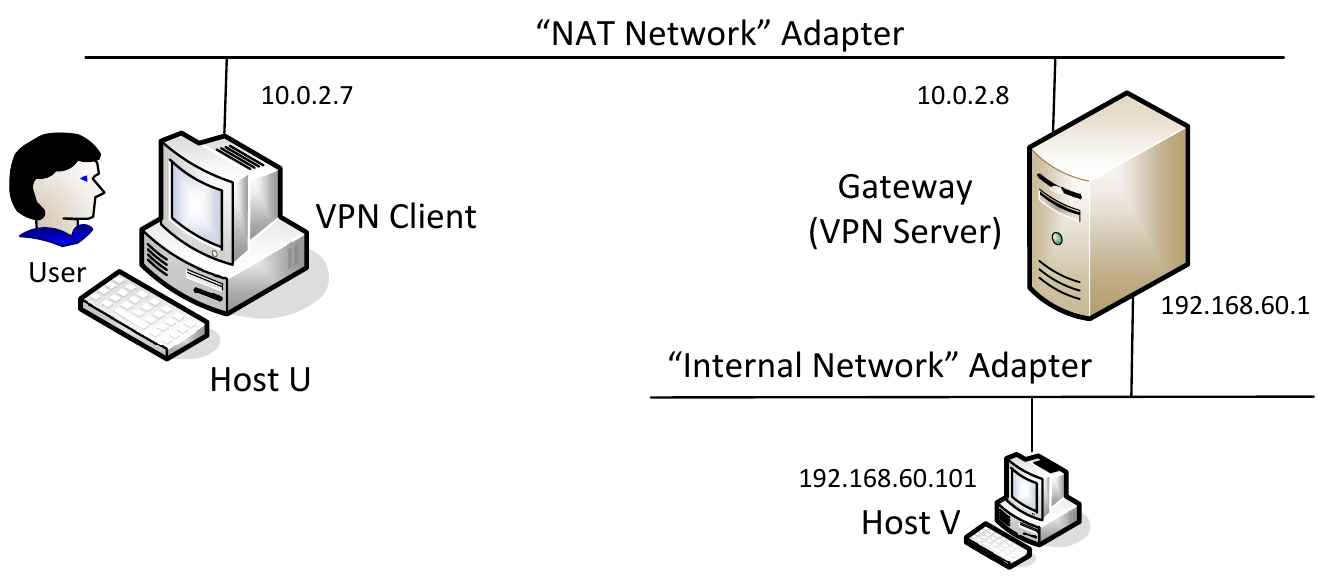
\includegraphics[scale=0.35]{t1_1.png}
    \end{center}{}
    \caption{VM setup for this lab}
    \label{fig:t1_1}
\end{figure}

Figure~\ref{fig:t1_1} shows the network graph of how the VM's should lay out. For redundancy, the IP address table is shown below:

\begin{center}
\begin{tabular}{ |c|c|c| } 
 \hline
 host & IP address(es) \\ 
 \hline
 client & 10.0.2.7  \\ 
 server & 10.0.2.8/192.168.60.1  \\ 
 target & 192.168.60.101 \\
 \hline
\end{tabular}
\end{center}

\subsubsection{Setting up NAT Network}
The first step to setting up the environment in virtualbox is to set up a NAT Network.


\begin{figure}[H]
    \begin{center}
        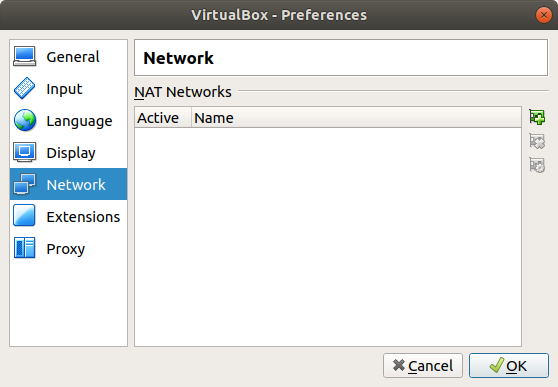
\includegraphics[scale=0.5]{NATNetwork_1.png}
    \end{center}{}
    \caption{VirtualBox Manager Preferences window}
    \label{fig:t1_2}
\end{figure}

Figure~\ref{fig:t1_2} shows the Virtualbox Manager Preferences window in which the Network tab is selected. Create a new NAT Network by clicking the green plus icon on the top right. 

\begin{figure}[H]
    \begin{center}
        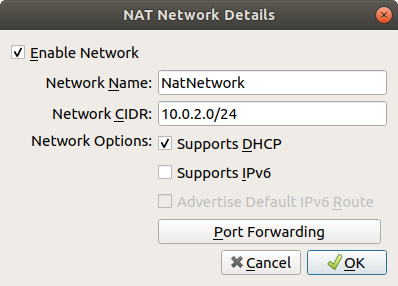
\includegraphics[scale=0.5]{NATNetwork_2.png}
    \end{center}{}
    \caption{Creating new NAT Network}
    \label{fig:t1_3}
\end{figure}

Figure~\ref{fig:t1_3} shows the window for creating a new NAT Network. Simply keep the defaults as they are and press OK.

\subsubsection{Setting up server settings}

\subsubsection{Setting up target settings}
\subsubsection{Setting up client settings}


\subsection{Task 2: Creating a VPN Tunnel using TUN/TAP}


\subsection{Task 3: Set up Routing on Client and Server VMs}
\subsection{Task 4: Authenticating the VPN Server}
\subsection{Task 5: Authenticating the VPN Client}
\subsection{Task 6: Supporting Multiple Clients}





% \subsubsection{Task 1 Displaying TLS Traffic in Wireshark}
% \subsubsection{Task 2 Getting IP Address from Hostname}
% \subsubsection{Task 3  Authentication Using the Shadow File}
% \subsubsection{Task 4 Inter-Process Communication Using Pipe}
% \subsubsection{Task 5 Using Select to Monitor Multiple Input Interfaces}
% \subsubsection{Task 6 An example: using telnet in our VPN}
% \subsubsection{Solution(s):}







\section{Conclusions}
VPN enables us to build a virtual private network over a public network, i.e. internet, such that connections with different users is protected regardless if the traffic goes through unprotected public networks.As shown in this lab, TSL/SSL provides privacy and data integrity between two or more communicating computer applications, i.e. client and sever. The connection is private because it uses symmetric cryptography to generate a shared secret key, which avoids the key distribution problem that other protocols encounter. 

\section{Future work and open problems}
\subsection{Future Work}
TSL/SSL VPN arose to solve the inability to support every multiple users while maintaining privacy. This protocol provides secure remote access via a web portal and nerwork-level access via SSL-secured tunnel between the client and network, with its main benefits of security and privacy. TSL/SSL VPN impacts future work drastically due to the growth of remote workforce, keeping employees connected to the work/academic applications they need and specifically for IT to ensure only authorized user gain access. 
\subsection{Open Problems}
\begin{itemize}
\item Implementation of TSL/SSL VPN requires products that support the current version of TLS because it is stronger than the older versions SSL. 
\end{itemize}
\begin{itemize}
\item An TSL/SSL VPN can attempt to ensure there is no carryover of sensitive information from session to session on a shared computer by wiping information, however it is not guarantee.
\end{itemize}


\section{Reference(s)}
\item Wenliang, D. (2019). "Chapter 12: Overview of Transport Layer Security".
\item 

\end{document}
